%%%%%%%%%%%%%%%%%%%%%%%%%%%%%%%%%%%%%%%%%
% Beamer Presentation
% LaTeX Template
% Version 1.0 (10/11/12)
%
% This template has been downloaded from:
% http://www.LaTeXTemplates.com
%
% License:
% CC BY-NC-SA 3.0 (http://creativecommons.org/licenses/by-nc-sa/3.0/)
%
%%%%%%%%%%%%%%%%%%%%%%%%%%%%%%%%%%%%%%%%%

%----------------------------------------------------------------------------------------
%	PACKAGES AND THEMES
%----------------------------------------------------------------------------------------

\documentclass{beamer}

\mode<presentation> {

% The Beamer class comes with a number of default slide themes
% which change the colors and layouts of slides. Below this is a list
% of all the themes, uncomment each in turn to see what they look like.

% \usetheme{default}
%\usetheme{AnnArbor}
%\usetheme{Antibes}
%\usetheme{Bergen}
% \usetheme{Berkeley}
% \usetheme{Berlin}
%\usetheme{Boadilla}
%\usetheme{CambridgeUS}
%\usetheme{Copenhagen}
%\usetheme{Darmstadt}
%\usetheme{Dresden}
%\usetheme{Frankfurt}
%\usetheme{Goettingen}
%\usetheme{Hannover}
%\usetheme{Ilmenau}
%\usetheme{JuanLesPins}
%\usetheme{Luebeck}
\usetheme{Madrid}
%\usetheme{Malmoe}
%\usetheme{Marburg}
%\usetheme{Montpellier}
% \usetheme{PaloAlto}
%\usetheme{Pittsburgh}
%\usetheme{Rochester}
% \usetheme{Singapore}
%\usetheme{Szeged}
% \usetheme{Warsaw}

% As well as themes, the Beamer class has a number of color themes
% for any slide theme. Uncomment each of these in turn to see how it
% changes the colors of your current slide theme.

%\usecolortheme{albatross}
%\usecolortheme{beaver}
%\usecolortheme{beetle}
%\usecolortheme{crane}
%\usecolortheme{dolphin}
%\usecolortheme{dove}
%\usecolortheme{fly}
%\usecolortheme{lily}
%\usecolortheme{orchid}
%\usecolortheme{rose}
%\usecolortheme{seagull}
%\usecolortheme{seahorse}
%\usecolortheme{whale}
%\usecolortheme{wolverine}

%\setbeamertemplate{footline} % To remove the footer line in all slides uncomment this line
%\setbeamertemplate{footline}[page number] % To replace the footer line in all slides with a simple slide count uncomment this line

%\setbeamertemplate{navigation symbols}{} % To remove the navigation symbols from the bottom of all slides uncomment this line
}

\usepackage{graphicx} % Allows including images
\graphicspath{{Images/}{../Images/}}
\usepackage{booktabs} % Allows the use of \toprule, \midrule and \bottomrule in tables
\usepackage{amsmath}

%----------------------------------------------------------------------------------------
%	TITLE PAGE
%----------------------------------------------------------------------------------------

\title[Intro to ML]{Introduction to Machine Learning} % The short title appears at the bottom of every slide, the full title is only on the title page

\author{Yixin Lin, Serge Assaad, Rohith Kuditipudi} % Your name
\institute[Duke] % Your institution as it will appear on the bottom of every slide, may be shorthand to save space
{
Duke University \\ % Your institution for the title page
\medskip
\textit{yixin.lin@duke.edu, serge.assaad@duke.edu, rohith.kuditipudi@duke.edu} % Your email address
}
\date{March 25, 2017} % Date, can be changed to a custom date

\begin{document}

\begin{frame}
\titlepage % Print the title page as the first slide
\end{frame}

\begin{frame}
\frametitle{Outline} % Table of contents slide, comment this block out to remove it
\tableofcontents % Throughout your presentation, if you choose to use \section{} and \subsection{} commands, these will automatically be printed on this slide as an overview of your presentation
\section{Overview of basic principles of machine learning}
\section{Introduction to neural networks}
\section{Tutorial on implementing deep learning algorithms}
\end{frame}


\begin{frame}{Overview of basic principles of machine learning}
\begin{itemize}
    \item Three components to any ML problem: the \textbf{task}, the \textbf{performance measure} and the \textbf{data}
    \item Essential definitions
    \begin{itemize}
        \item \textbf{Features}
        \item \textbf{Model}
        \item \textbf{Parameters}
        \item \textbf{Loss}
        
    \end{itemize}
    \item Two (broad) kinds of tasks
    \begin{itemize}
        \item \textbf{Supervised learning}: data is labeled/annotated
        \item \textbf{Unsupervised learning}: data is unlabeled 
    \end{itemize}
    
\end{itemize}
    
\end{frame}

\begin{frame}{Example: Linear Regression}
\begin{itemize}
    \item Can we \textbf{predict} y given x, using the model $\hat{\textbf{y}}=m\textbf{x}+\textbf{b}$?
    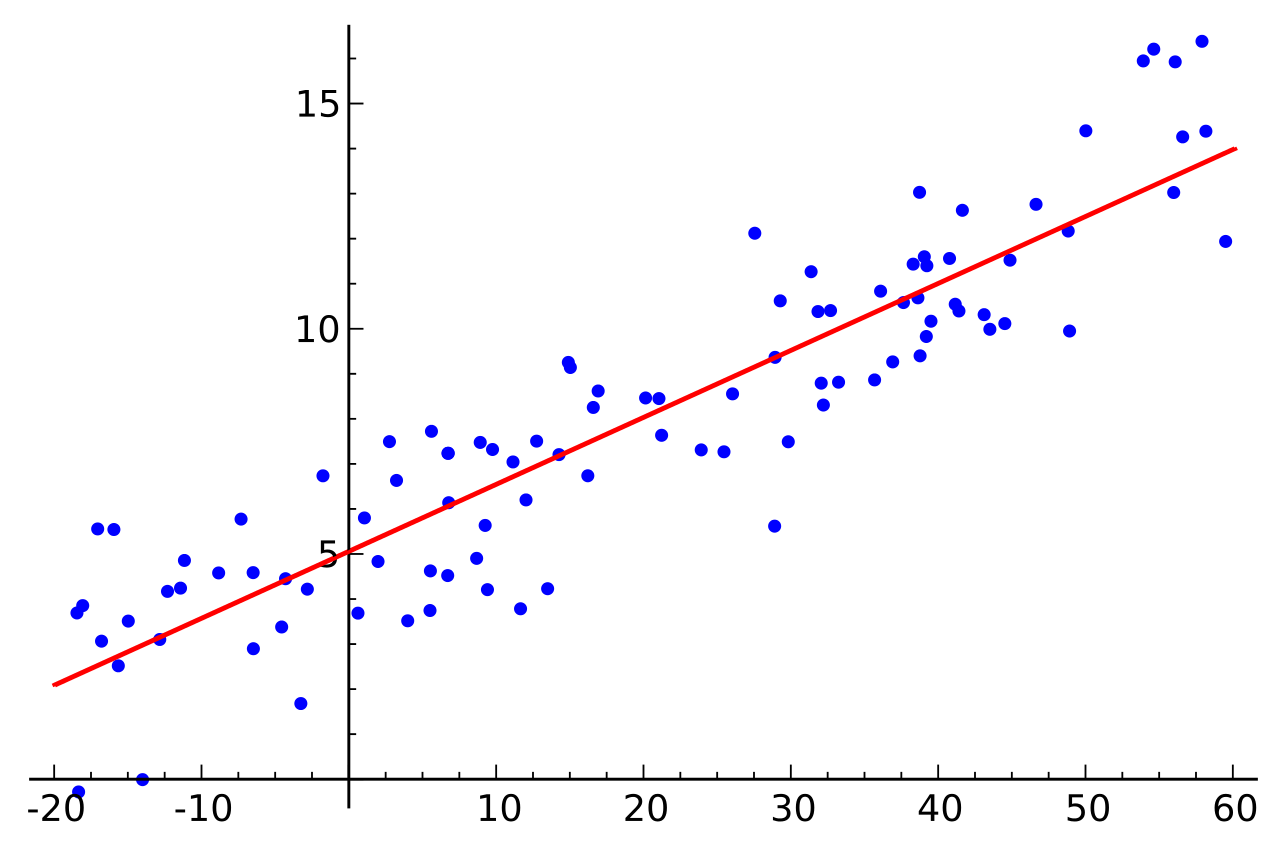
\includegraphics[scale=0.2]{LinReg.png}

\end{itemize}

\end{frame}

\begin{frame}{Introduction to Neural Networks}
\begin{itemize}
    \item Neurons are the building blocks of neural networks
    \item Each neuron is a \textbf{function}: $y=f(\textbf{w}^{T}\textbf{x}+\textbf{b})$
    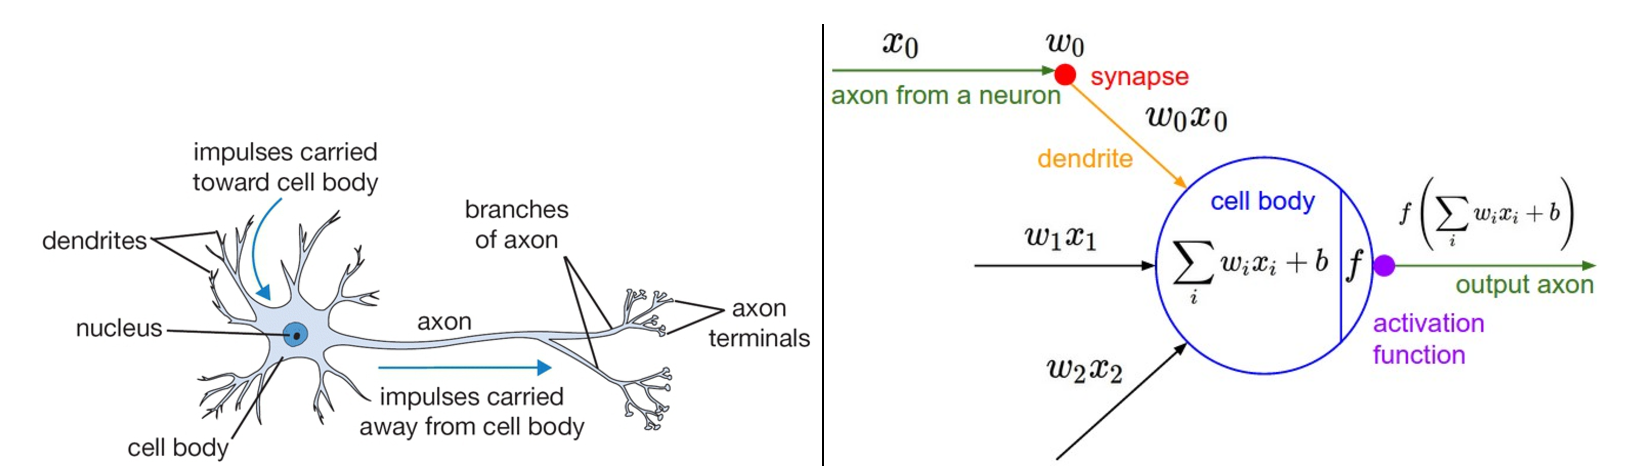
\includegraphics[scale=0.4]{Neuron.png}
    \item Note: \textbf{neural networks $\neq$ neuroscience!!!!!}
\end{itemize}
\end{frame}

\begin{frame}{Neural Networks are Layers of Neurons}
    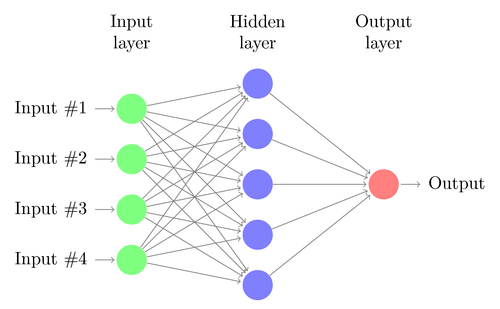
\includegraphics[scale=0.6]{neural-network.png}
\end{frame}

\begin{frame}{What are Neural Networks Good For?}
    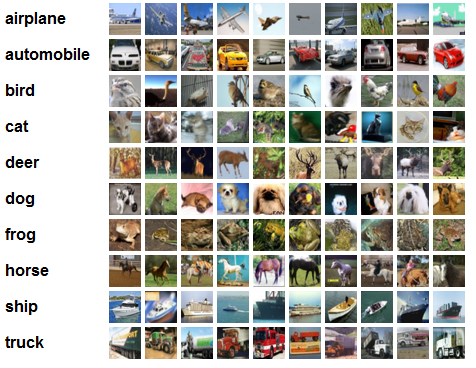
\includegraphics[scale=0.7]{cifar_preview.png}
\end{frame}

\begin{frame}{Training Neural Networks: Gradient Descent}
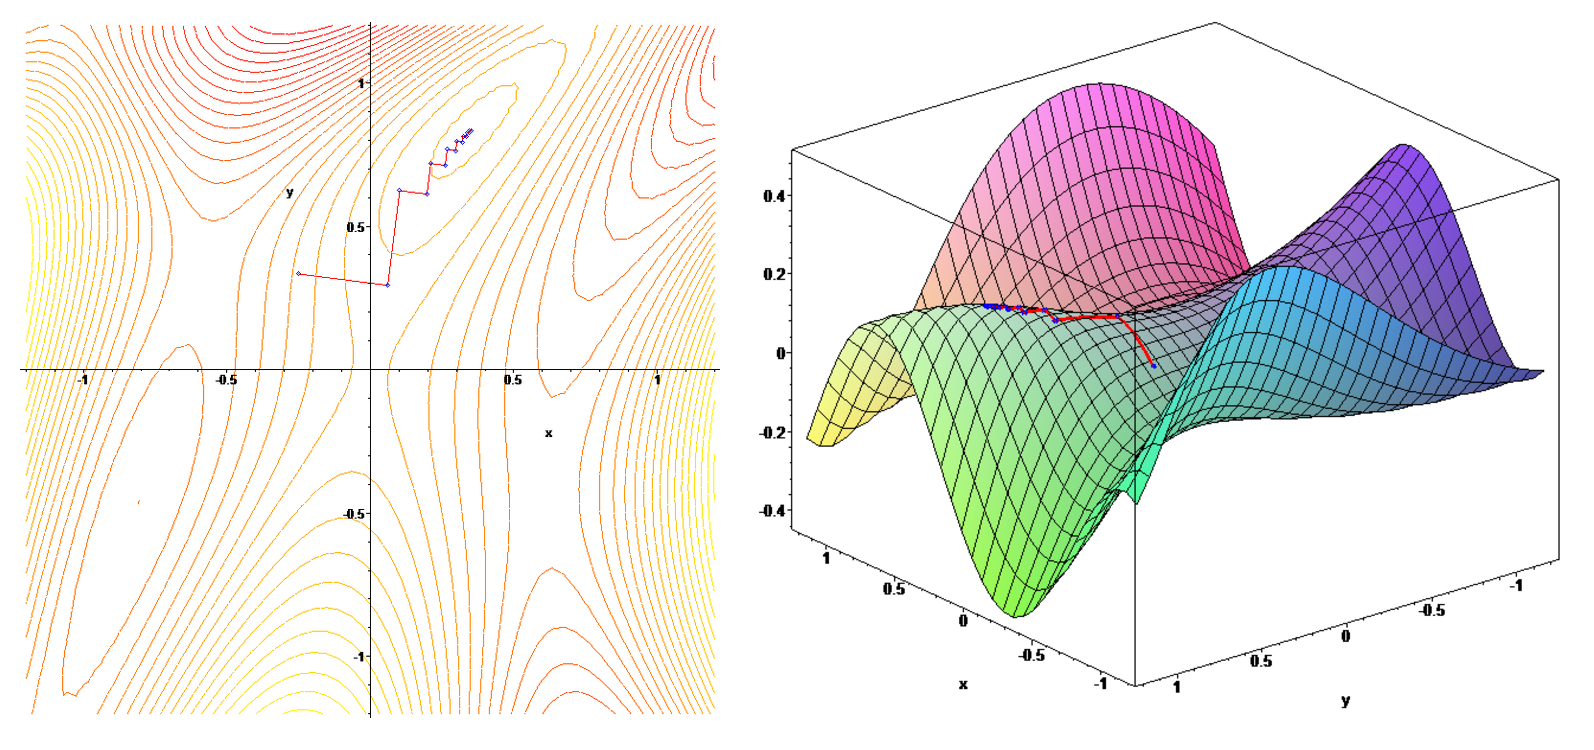
\includegraphics[scale=0.4]{gradient.png}
\end{frame}

\begin{frame}{Tutorial}
\begin{itemize}
    \item Time to \textbf{build something}!
    \item Goals:
      \begin{itemize}
        \item Give you a basic framework for thinking about what machine learning is and isn't
        \item Have a project done or almost done at the end of the workshop
        \item Get you set up to continue to tinker and play with machine learning models
      \end{itemize}
\end{itemize}

\end{frame}

\begin{frame}
\Huge{\centerline{Thanks!}}

\Large{\centerline{Resources and references: \href{http://yixinlin.net/intro-ml}{yixinlin.net/intro-ml}}}

\end{frame}

%----------------------------------------------------------------------------------------

\end{document} 
